\subsection{Studies of noise peak movement under temperature variation}
\label{sipmNoiseMovement}
Since we are using SiPMs with a sensitive area of $3\times3\,\mathrm{mm}$ we discovered a clipping in our frontend electronics due to higher signals. Therefore we had to set down the amplification factor. This implicates that individual p.e. peaks were not observable anymore and the possiblity to regulated the bias voltage on temperature variation by measuring the asymmetry of the edges of the first p.e. to keep it on a constant value could not be realized in that way. The following studies were done to check if a implementation of this algorithm on the entire noise peak could be possible.

\subsubsection{Experimental setup}
To measure the movement of the noise peak under temperature variation a prototyp frontend described in chapter REF TO LARS was used without scintillator.
The temperature regulation was was done in a cooling box which could be regulated with the temperature device located between the two SiPMs. The bias voltage supplied to the SiPM was fixed to the constant value of the default voltage given by the producer Hamamatsu. The spectra based on the peakheights was collected from pulses taken with an CAEN VX1721 8-bit FADC. Thereby the peakheights were defined as the potential difference between the pulse maximum and the average baseline. 
The FADC was triggers itselves on pulses over $0.5\,\mathrm{p.e.}$. To avoid influence from pedestals only one SiPM-Channel was regarded. To analyse the peak a fit of an exponentially modified gaussian distribution was used due to best match to the shape. In figure \ref{NoiseMoveExample} a spectrum example is shown with one of these fits.
\begin{figure}[h]
	\centering
	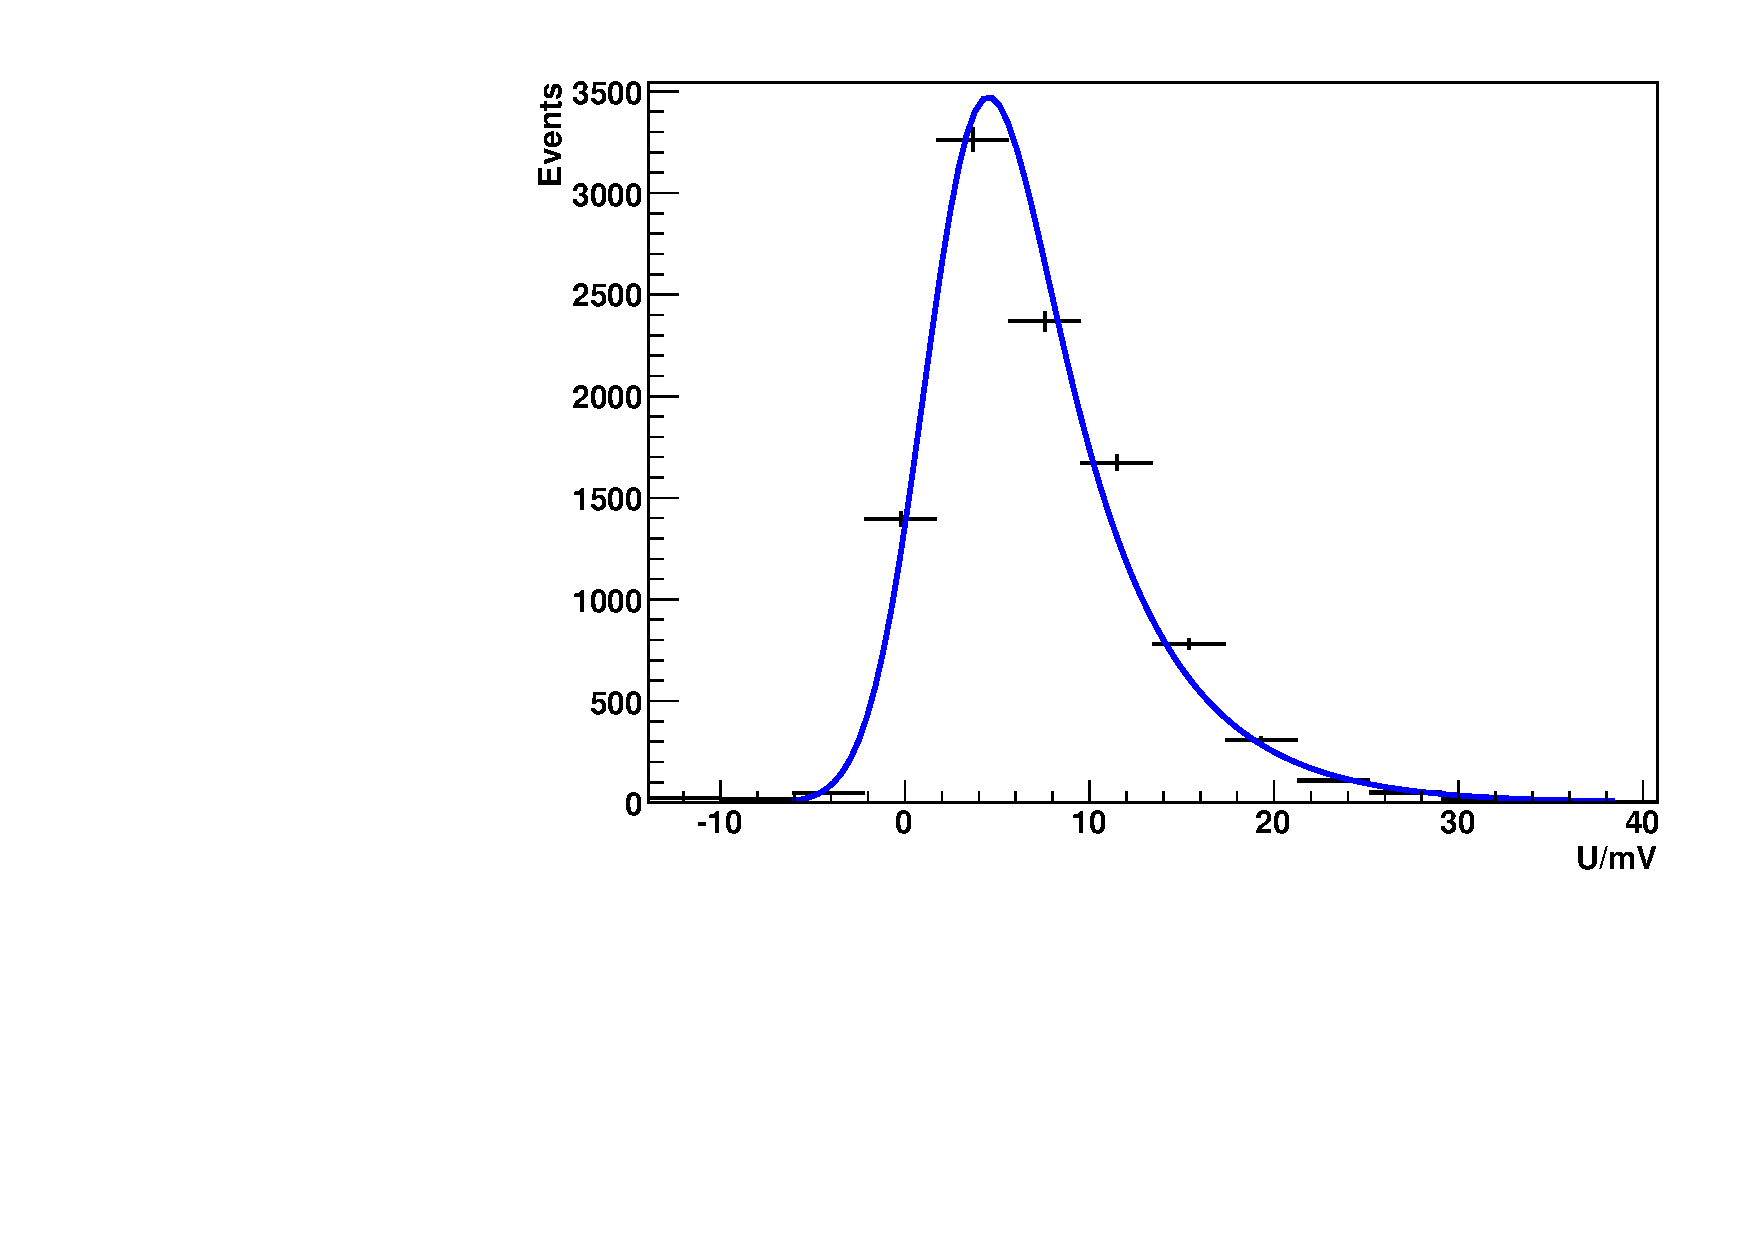
\includegraphics[width = .65\textwidth]{Figures/radermacher/NoiseMovementExample.pdf}
	\caption{Example for peakheightspectrum with exponentially modified gaussian fit}
	\label{NoiseMoveExample}
\end{figure}
\subsubsection{Results}
Figure \ref{NoiseMove} shows the results of the noise peak movement. The mean of the noise peak shifts linear to smaller peakheights with increasing temperature. This is based on the decreasing overvoltage which is supplied by keeping the bias voltage constant. 
This also causes the peak width getting smaller because the gain drops with this decreasing overvoltage. Based on this results the possiblity to adjust the bias voltage by the movement of the noise peak is given but further studies on the comparator windows have to be done due to the non symmetrical distribution. 
\begin{figure}[h]
	\centering
	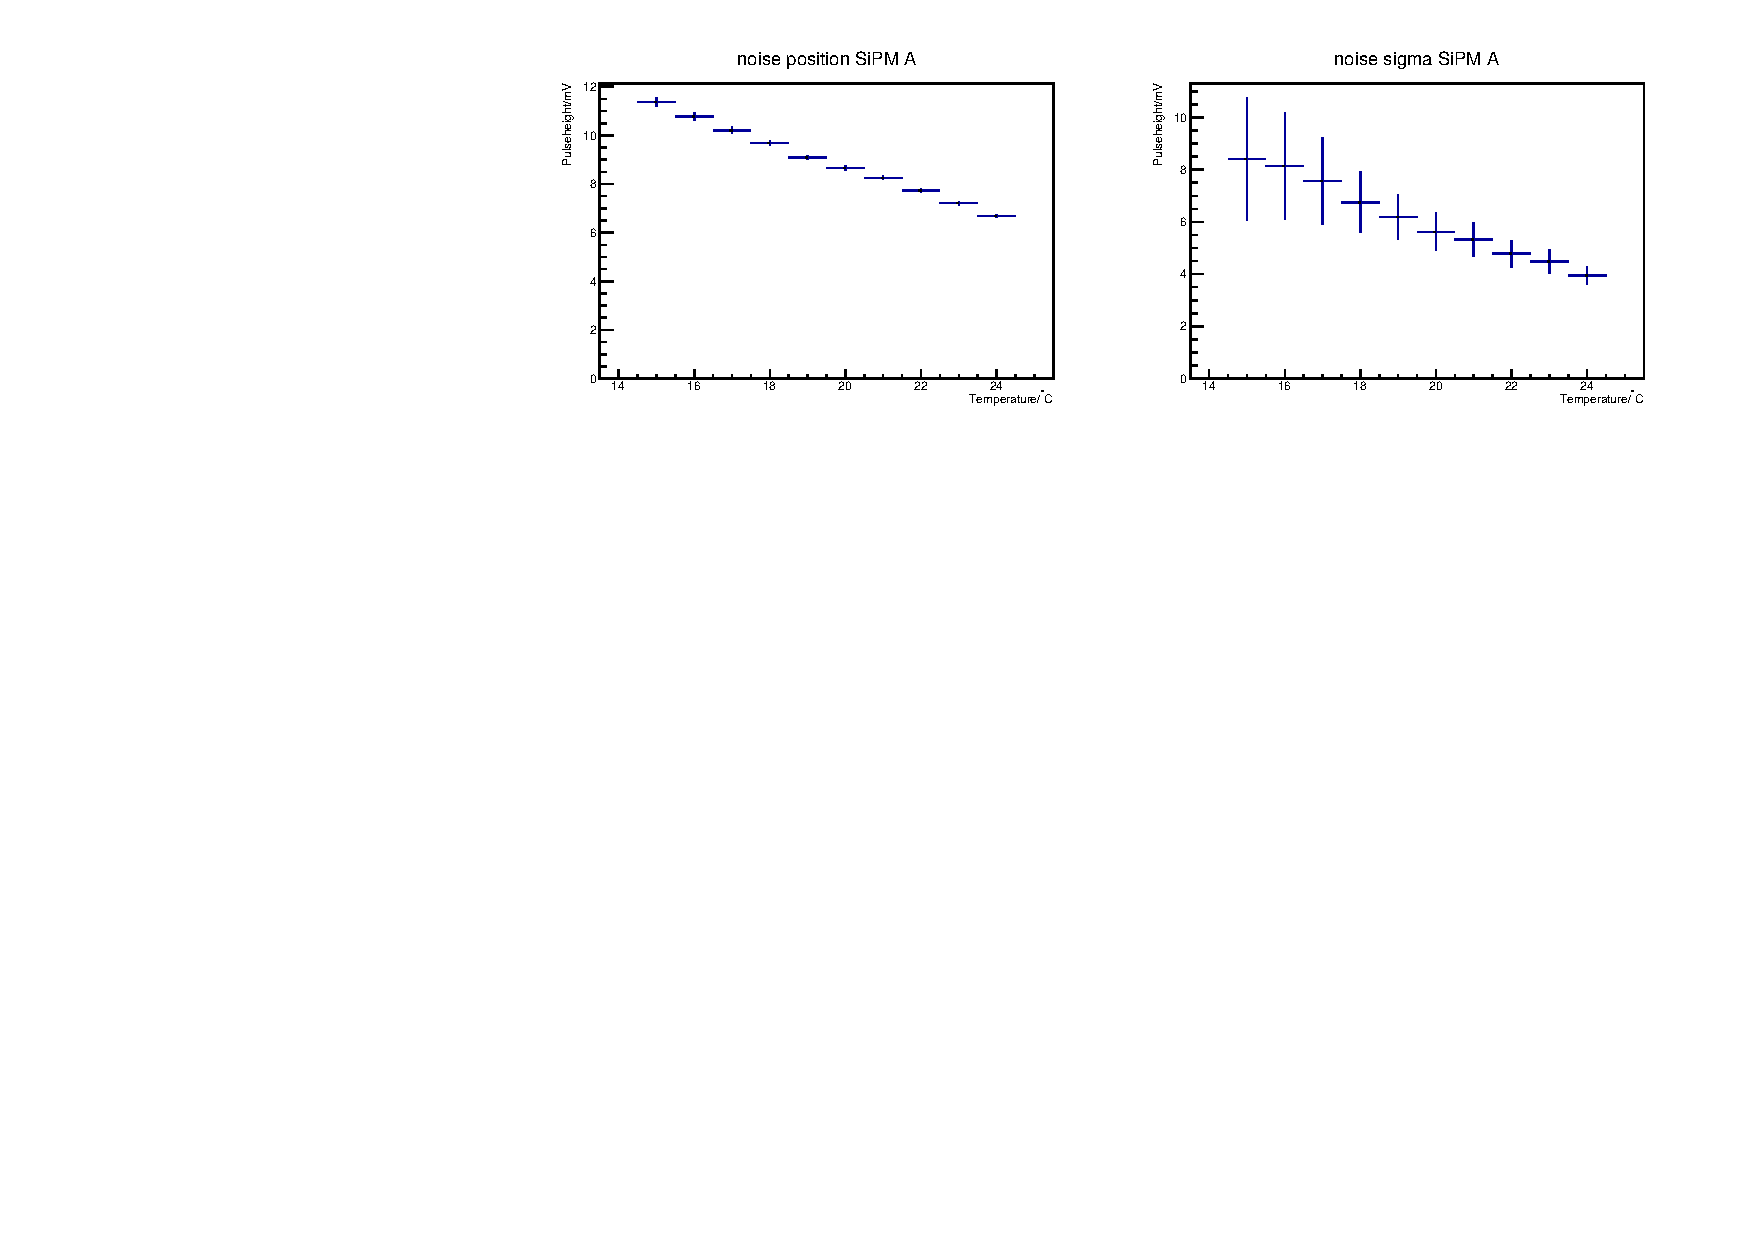
\includegraphics[width = .99\textwidth]{Figures/radermacher/result_ExpGauOnlySipmATriggerNEW.pdf}
	\caption{measurement of noise peak movement}
	\label{NoiseMove}
\end{figure}
